%!TEX encoding = UTF-8 Unicode
\documentclass[12pt]{article} 
\usepackage{CJK}
\usepackage{graphicx}
\usepackage{mathtools}
\usepackage{mathrsfs}
\usepackage{amssymb}
\usepackage[
  letterpaper,%
  textheight={47\baselineskip+\topskip},%
  textwidth={\paperwidth-100pt},%
  footskip=75pt,%
  marginparwidth=0pt,%
  top={\topskip+0.75in}]{geometry}

\begin{CJK}{UTF8}{bsmi}
\title{Machine Learning Assignment 01}
\author{103061527 李豪韋}
\date{}

\begin {document}
\maketitle
	\begin {enumerate}
		%%%%%%%%%%%%%%%                           Q1                                    %%%%%%%%%%%%%%%
		\item What is the difference in terms of the performance between hypotheses based on the objective 
			arg$_\theta$ min $\displaystyle\sum_{t=1}^N [r^{(t)}-h(x^{(t)};\theta)]^2$ and 
			arg$_\theta$min$\displaystyle\sum_{t=1}^N|r^{(t)}-h(x^{(t)};\theta)|$ respectively?
			
			% Here's the answer
			\noindent\makebox[\linewidth]{\rule{\textwidth}{0.4pt}}
			\begin {flushleft} % Insert the answer
				$[r^{(t)}-h(x^{(t)};\theta)]^2$ has an analytic form that makes finding solutions easier, 
				but suffers from difference accuracy issue. $|r^{(t)}-h(x^{(t)};\theta)|$ cannot be differentiated directly, 
				but can estimate difference in a more accurate way.
			\end {flushleft}
			\noindent\makebox[\linewidth]{\rule{\textwidth}{0.4pt}}
			
		%%%%%%%%%%%%%%%                           Q2                                    %%%%%%%%%%%%%%%
		\item In logistic regression, show that $l(\beta)$ = 
			$\displaystyle\sum_{t=1}^N\{y^{(t)}\beta^T\widetilde{x}^{(t)}-log(1+e^{\beta^T\widetilde{x}^{(t)}})\}$.
		
			% Here's the answer
			\noindent\makebox[\linewidth]{\rule{\textwidth}{0.4pt}}
			\begin {flushleft}% Insert the answer
			
				\begin {align*}
					l(\beta) & = log( p( y | \widetilde{x} ; \beta ) ) = log\bigg(
					\displaystyle\prod_{t=1}^N ( \pi ( \widetilde{x}^{(t)} ; \beta ) )^{ y^{(t)} } 
					( 1 - \pi ( \widetilde{x}^{(t)} ; \beta ) )^{ ( 1 - y^{(t)} ) }
					\bigg) \\
					& = \displaystyle\sum_{t=1}^N y^{(t)} log( \pi ( \widetilde{x}^{(t)} ; \beta ) ) +
					\displaystyle\sum_{t=1}^N (1 - y^{(t)}) log(1 - \pi ( \widetilde{x}^{(t)} ; \beta ) ) \\
					& = \displaystyle\sum_{t=1}^N y^{(t)} log( \frac{1}{1 + \exp{(- \beta^T \widetilde{x}^{(t)} )}} ) + 
					\displaystyle\sum_{t=1}^N (1 - y^{(t)}) 
					log( \frac{ \exp{ ( -\beta^T \widetilde{x}^{(t)} ) } }{ 1 + \exp{ ( -\beta^T \widetilde{x}^{(t)} ) } } ) \\
					& = \displaystyle\sum_{t=1}^N y^{(t)} \beta^T \widetilde{x}^{(t)}  -
					\displaystyle\sum_{t=1}^N log( 1 + \exp{ ( \beta^T \widetilde{x}^{(t)} ) } )
				\end {align*}	
				
			\end {flushleft}
			\noindent\makebox[\linewidth]{\rule{\textwidth}{0.4pt}}
			
		%%%%%%%%%%%%%%%                           Q3                                    %%%%%%%%%%%%%%%
		\item Read Appendix C on the definitions of convex set and functions.
			\begin {enumerate}
				%%%%%%%%%%%                           (a)                                   %%%%%%%%%%%
				\item Show that the intersection of convex sets, 
					$\displaystyle\bigcap_{i \in N}C_i$ where $C_i \subseteq \mathbb{R}^n$, is convex.
				
					% Here's the answer
					\noindent\makebox[\linewidth]{\rule{\textwidth}{0.4pt}}
					\begin {flushleft} % Insert the answer 
					
						Let $x, y \in \displaystyle\bigcap_{i \in N}C_i$, then $\forall k \in N, \quad x, y \in C_k$ \\
						By definition, $(1 - \theta)x + \theta y \in C_k, \quad \forall k \in N, \quad \theta \in [0, 1]$ \\
						And because $(1 - \theta)x + \theta y \in C_k, \quad \forall k \in N, \quad \theta \in [0, 1]$ \\
						Hence $(1 - \theta)x + \theta y \in \displaystyle\bigcap_{i \in N}C_i, \quad \theta \in [0, 1]$ \\
						Therefore, $ \displaystyle\bigcap_{i \in N}C_i $ is also a convex.
					
					\end {flushleft}
					\noindent\makebox[\linewidth]{\rule{\textwidth}{0.4pt}}
					
				%%%%%%%%%%%                           (b)                                   %%%%%%%%%%%	
				\item Show that the log-likelihood function for logistic regression, $l(\beta)$, is concave.
				
					% Here's the answer
					\noindent\makebox[\linewidth]{\rule{\textwidth}{0.4pt}}
					\begin {flushleft} % Insert the answer
					
						Let $\beta \subseteq \mathbb{F}^{n \times 1}$, which is a vector space whose elements 
						are contained by a field $\mathbb{F}$, where $n$ is the dimension of 
						$x^{(t)} \quad \forall t \in [1, N], t \in \mathbb{N}$. Obviously, vector spaces are convex. \\
						Define $f(\beta; v)$ = $- \langle \beta, v \rangle$ = $-\beta^Tv$, 
						where $v \in \mathbb{F}^{n \times 1}$. \\
						Because of linearity of matrix computation, we have \\
						\begin {align*}
							f(\theta x + (1-\theta)y; v) = -\langle \theta x + (1-\theta)y, v \rangle
							& = -(\theta \langle x, v \rangle + (1-\theta) \langle y, v \rangle) \\
							& = \theta f(x; v) + (1-\theta) f(y; v) \\
							& \leq \theta f(x; v) + (1-\theta) f(y; v) \quad \forall x, y \in \beta \quad \theta \in [0, 1]
						\end {align*}
						Hence $f: \mathbb{F}^{n \times 1} \to \mathbb{F}$ is convex. \\
						Define $g(v)$ = $log(1+e^v)$ where $v \in \mathbb{F}$, and $v$ can be expressed as 
						$\theta x + (1-\theta)y$ where $x, y \in \mathbb{F} \quad \theta \in [0, 1]$, then
						\begin{align*}
							g(\theta x + (1-\theta)y)
							& = log(1+e^{ (\theta x + (1-\theta)y) }) \\
							& \leq log (1 + e^{\theta x} + e^{(1-\theta)y} + e^{\theta x + (1-\theta)y}) \\
							& = log \big( (1 + e^{\theta x})(1 + e^{(1-\theta)y}) \big) \\
							& \leq log \big( (1 + e^x)^\theta (1 + e^y)^{(1-\theta)} \big) \\
							& = \theta log(1 + e^x) + (1-\theta) log(1 + e^y) \\
							& = \theta g(x) + (1-\theta) g(y)
						\end{align*}
						Hence $g: \mathbb{F} \to \mathbb{F}$ is convex. \\
						Then consider $-l(\beta)$:
						\begin {center}
							$-l(\beta)$ = $-\displaystyle\sum_{t=1}^N y^{(t)} \beta^T x^{(t)}  +
								\displaystyle\sum_{t=1}^N log( 1 + \exp{ ( \beta^T x^{(t)} ) } )$ 
								= $\displaystyle\sum_{t=1}^N \bigg[ y^{(t)} f(\beta; x^{(t)}) + g(f(\beta; x^{(t)})) \bigg]$
						\end {center}
						$y^{(t)} f(\beta; x^{(t)})$ is convex $\forall t \in [1, N], t \in \mathbb{N} \quad$
						($\because y^{(t)}$ is a scalar with the value of either 1 or 0). 
						In addition, $g(f(\beta; v))$ is also convex because it is 
						the convex function of a convex set. Therefore, $-l(\beta)$ is convex because it can be expressed 
						as a summation of convex sets. \\
						Hence, $l(\beta)$ is concave.
					
					\end {flushleft}
					\noindent\makebox[\linewidth]{\rule{\textwidth}{0.4pt}}
					
					
			\end {enumerate}
		
		%%%%%%%%%%%%%%%                           Q4                                    %%%%%%%%%%%%%%%
		\item Consider the locally weighted linear regression problem with the following objective:\\ 
			\begin{center}
				arg $\underset{w \in \mathbb{R}^{d+1}}{min} \frac{1}{2} \displaystyle\sum_{i=1}^Nl^{(i)}(w^T 
				\bigg[ \begin{array}{c}1 \\ x^{(i)}\end{array} \bigg] - r^{(i)})^2$
			\end{center} 
			local to a given instance $x'$ whose label will be predicted, where $l^{(i)}$ = 
			$\exp{(- \frac{(x' - x^{(i)})^2}{2 \tau^2})}$ 
			
			\begin {enumerate}
				%%%%%%%%%%%                           (a)                                   %%%%%%%%%%%
				\item Show that the above objective can be written as the form \\
					\begin {center} $(Xw-r)^TL(Xw-r)$. \end {center}	
					Specify clearly what $X$, $r$, and $L$ are.
					
					% Here's the answer
					\noindent\makebox[\linewidth]{\rule{\textwidth}{0.4pt}}
					\begin {flushleft} % Insert the answer
					
						$\frac{1}{2}\displaystyle\sum_{t=1}^N l^{(i)}$ 
							$(w^T \bigg[ \begin{array}{c}1 \\ x^{(i)}\end{array} \bigg] - r^{(i)})^2$ = 
							$\langle A$, $B \rangle$ \\
						$A = 
						\begin{pmatrix}
							1 & x_1^{(1)} & \cdots & x_d^{(1)} \\
							1 & x_1^{(2)} & \cdots & x_d^{(2)} \\
							\vdots & \vdots & \ddots & \vdots \\
							1 & x_1^{(N)} & \cdots & x_d^{(N)}
						\end{pmatrix}
						\begin{pmatrix}
							w_0 \\ w_1 \\ \vdots \\ w_d
						\end{pmatrix} - 
						\begin{pmatrix}
							r^{(1)} \\ r^{(2)} \\ \vdots \\ r^{(N)}
						\end{pmatrix}$ = $Xw-r$ \\
						\begin{align*}
							B & = \frac{1}{2} \Bigg[
							\begin{pmatrix}
								l^{(1)}(1 & x_1^{(1)} & \cdots & x_d^{(1)}) \\
								l^{(2)}(1 & x_1^{(2)} & \cdots & x_d^{(2)}) \\
								\vdots & \vdots & \vdots & \vdots \\
								l^{(N)}(1 & x_1^{(N)} & \cdots & x_d^{(N)})
							\end{pmatrix}
							\begin{pmatrix}
								w_0 \\ w_1 \\ \vdots \\ w_d
							\end{pmatrix} - 
							\begin{pmatrix}
								l^{(1)}r^{(1)} \\ l^{(2)}r^{(2)} \\ \vdots \\ l^{(N)}r^{(N)}
							\end{pmatrix} \Bigg] \\
							& = 
							\begin{pmatrix}
								\frac{ l^{(1)} }{2} & 0 & \cdots & 0 \\
								0 & \frac{ l^{(2)} }{2} & \cdots & 0 \\
								\vdots & \vdots & \ddots & \vdots \\
								0 & 0 & \cdots & \frac{ l^{(N)} }{2}
							\end{pmatrix} \Bigg[
							\begin{pmatrix}
								1 & x_1^{(1)} & \cdots & x_d^{(1)} \\
								1 & x_1^{(2)} & \cdots & x_d^{(2)} \\
								\vdots & \vdots & \ddots & \vdots \\
								1 & x_1^{(N)} & \cdots & x_d^{(N)}
							\end{pmatrix}
							\begin{pmatrix}
								w_0 \\ w_1 \\ \vdots \\ w_d
							\end{pmatrix} - 
							\begin{pmatrix}
								r^{(1)} \\ r^{(2)} \\ \vdots \\ r^{(N)}
							\end{pmatrix} \Bigg] \\
							& = L(Xw-r)
						\end{align*}
						Hence: \\ 
						$X^{(t)}$ = $\begin{pmatrix} 1 & x^{(t)} \end{pmatrix}$, $\forall t \in [1, N] \quad t \in \mathbb{N}$ \\
						$r_t$ = $r^{(t)}$, $\forall t \in [1, N] \quad t \in \mathbb{N}$ \\
						$L_{ij}$ = $\frac{ l^{(i)} }{ 2 } \delta_{ij}$, $\forall i, j \in [1, N] \quad i, j \in \mathbb{N}$ 
						(i.e. L is a diagonal matrix, $L_{ii}$ = $\frac{ l^{(i)} }{ 2 }$)
						
					\end {flushleft}
					\noindent\makebox[\linewidth]{\rule{\textwidth}{0.4pt}}
					
				%%%%%%%%%%%                           (b)                                   %%%%%%%%%%%	
				\item Give a close form solution to $w$. 
					(Hint: recall that we have $w = (X^TX)^{-1}X^Tr$ in linear regression when $l^{(i)}$ = 1 for all $i$)
					
					% Here's the answer
					\noindent\makebox[\linewidth]{\rule{\textwidth}{0.4pt}}
					\begin {flushleft} % Insert the answer
						Find $w_{exm}$ such that $\bigtriangledown\bigg[\frac{1}{2}\displaystyle\sum_{t=1}^N l^{(i)}$
						$(w^T \bigg[ \begin{array}{c}1 \\ x^{(i)}\end{array} \bigg] - r^{(i)})^2\bigg]
						\Bigg|_{w=w_{exm}}$ = 0.
						
						\begin{align*}
							(Xw-r)^TL(Xw-r) & = (w^TX^T - r^T)L(Xw-r) \\
							& = w^TX^TLXw - w^TX^TLr - r^TLXw + r^TLr \\
							\bigtriangledown \bigg[ (Xw-r)^TL(Xw-r) \bigg]
							& = \bigtriangledown (w^TX^TLXw - w^TX^TLr - r^TLXw + r^TLr) \\
							& = 2X^TL^TXw - X^TLr - X^TL^Tr \\
							& = 2 (X^TLXw - X^TLr) \\
							2 (X^TLXw_{exm} - X^TLr) = 0 
							& \implies w_{exm} = (X^TLX)^{-1}(X^TL)r
						\end{align*}
					
					\end {flushleft}
					\noindent\makebox[\linewidth]{\rule{\textwidth}{0.4pt}}
					
				%%%%%%%%%%%                           (c)                                   %%%%%%%%%%%
				\item Suppose that the training examples $(x^{(i)}, r^{(i)})$ are i.i.d. 
					samples drawn from some joint distribution with the marginal: \\
					\begin {center}
						$p(r^{(i)} | x^{(i)} ; w)$ = $\frac{1}{\sqrt{2\pi\sigma^{(i)}}}$ $\exp{\Bigg(
							- \frac{(r^{(i)} - w^T\bigg[ \begin{array}{c} 1 \\ x^{(i)} \end{array} \bigg])^2}{2\sigma^{(i)2}}
						\Bigg)}$
					\end {center}
					where $\sigma^{(i)}$'s are constants. Show that finding the maximum likelihood of $w$ reduces to 
					solving the locally weighted linear regression problem above. Specify clearly what the $l^{(i)}$ is 
					in terms of the $\sigma^{(i)}$'s.
					
					% Here's the answer
					\noindent\makebox[\linewidth]{\rule{\textwidth}{0.4pt}}
					\begin {flushleft} % Insert the answer
						
						Suppose the transformation from dataset to label can be expressed as: \\
							\begin{center}
								$r^{(i)}$ = $h(x^{(i)} ; w) + \epsilon$, where $h(x^{(i)} ; w)$ = $w^T
								\bigg[ \begin{array}{c} 1 \\ x^{(i)} \end{array} \bigg]$ 
								and $\epsilon \sim \mathscr{N} (0, \sigma)$.
							\end{center}
							\begin{align*}
								log \big( p(r\big|x;w) \big) & = log \big( p(h(x ; w) + \epsilon\big|x;w) \big) \\
								& = log \big( \displaystyle\prod_{x^{(i)} \in x} p (h(x^{(i)} ; w) + \epsilon\big|x^{(i)};w) \big) \\
								& = log \bigg( (\frac{1}{ \sqrt{2\pi\sigma^{(i)} } })^{|x|} 
								\displaystyle\prod_{x^{(i)} \in x} \exp{ \big( -
								\frac{ \big(r^{(i)}-h(x^{(i)} ; w)\big)^2 }{ 2\sigma^{(i)2} } \big) } \bigg) \\
								& = O \bigg( -\displaystyle\sum_{ x^{(i)} \in x } \frac{ \big(r^{(i)}-h(x^{(i)} ; w)\big)^2 }
								{ 2\sigma^{(i)2} } \bigg) \\
								& = O \bigg( -\frac{1}{2} \displaystyle\sum_{ x^{(i)} \in x } 
								l^{(i)} \big(r^{(i)}-w^T \bigg[ \begin{array}{c} 1 \\ x^{(i)} \end{array} \bigg] \big)^2 \bigg) \\
								& \implies l^{(i)} = -\frac{ 1 }{ \sigma^{ (i)2 } }
							\end{align*}
						
					\end {flushleft}
					\noindent\makebox[\linewidth]{\rule{\textwidth}{0.4pt}}
					
				%%%%%%%%%%%                           (d)                                   %%%%%%%%%%%
				\item Implement a linear regressor (see the spec for more details) on the provided 1D dataset. \\
					Plot the data and your fitted line. (Hint: don't forget the intercept term)
					
					% Here's the answer
					\noindent\makebox[\linewidth]{\rule{\textwidth}{0.4pt}}
					\begin {flushleft} % Insert the answer
						The regression is implemented with LMS algorithm.
						\begin{center}
							$w$ = $\arg$ $\displaystyle \min_{w \in \mathbb{R}^{2 \times 1}}$
							$\bigg\| 
							\begin{pmatrix}
								1 & x^{(1)} \\
								1 & x^{(2)} \\
								\vdots & \vdots \\
								1 & x^{(N)}
							\end{pmatrix}
							\begin{pmatrix}
								w^{(1)} \\ w^{(2)}
							\end{pmatrix} - 
							\begin{pmatrix}
								y^{(1)} \\ y^{(2)} \\ \vdots \\ y^{(N)}
							\end{pmatrix}
							\bigg\|^2$
						\end{center}
						\begin{center}
							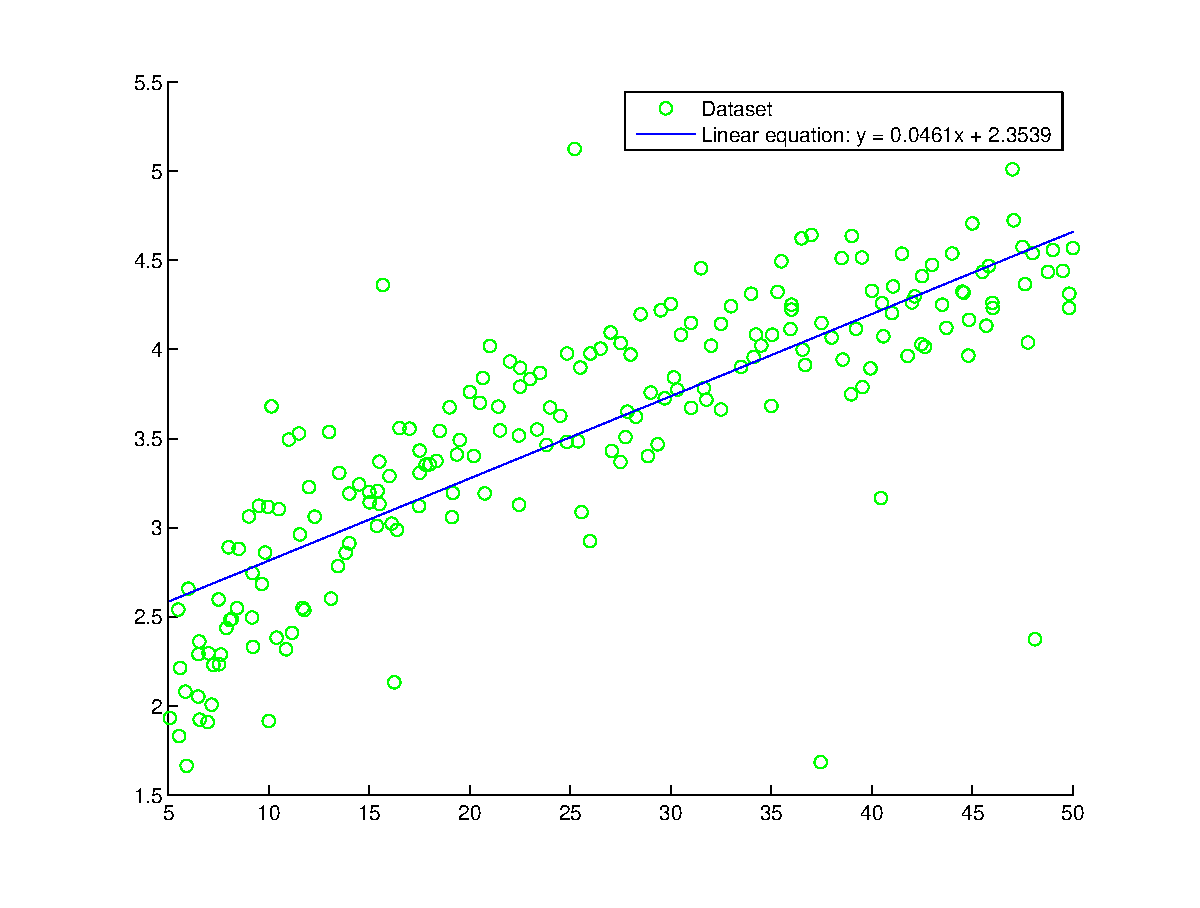
\includegraphics[scale = 0.6]{Q4_d}
						\end{center}
						\begin{center}
							Line equation: $y$ = $0.0461x + 2.3539$, MSE = 0.1971.
						\end{center}
					\end {flushleft}
					\noindent\makebox[\linewidth]{\rule{\textwidth}{0.4pt}}
					
				%%%%%%%%%%%                           (e)                                   %%%%%%%%%%%
				\item Implement 4 locally weighted linear regressors (see the spec for more details) on the same 
					dataset with $\tau$ = 0.1, 1, 10, and 100 respectively. Plot the data and your 4 fitted curves.
					(for different $x'$'s within the dataset range).
					
					% Here's the answer
					\noindent\makebox[\linewidth]{\rule{\textwidth}{0.4pt}}
					\begin {flushleft} % Insert the answer
						%\begin{center}
							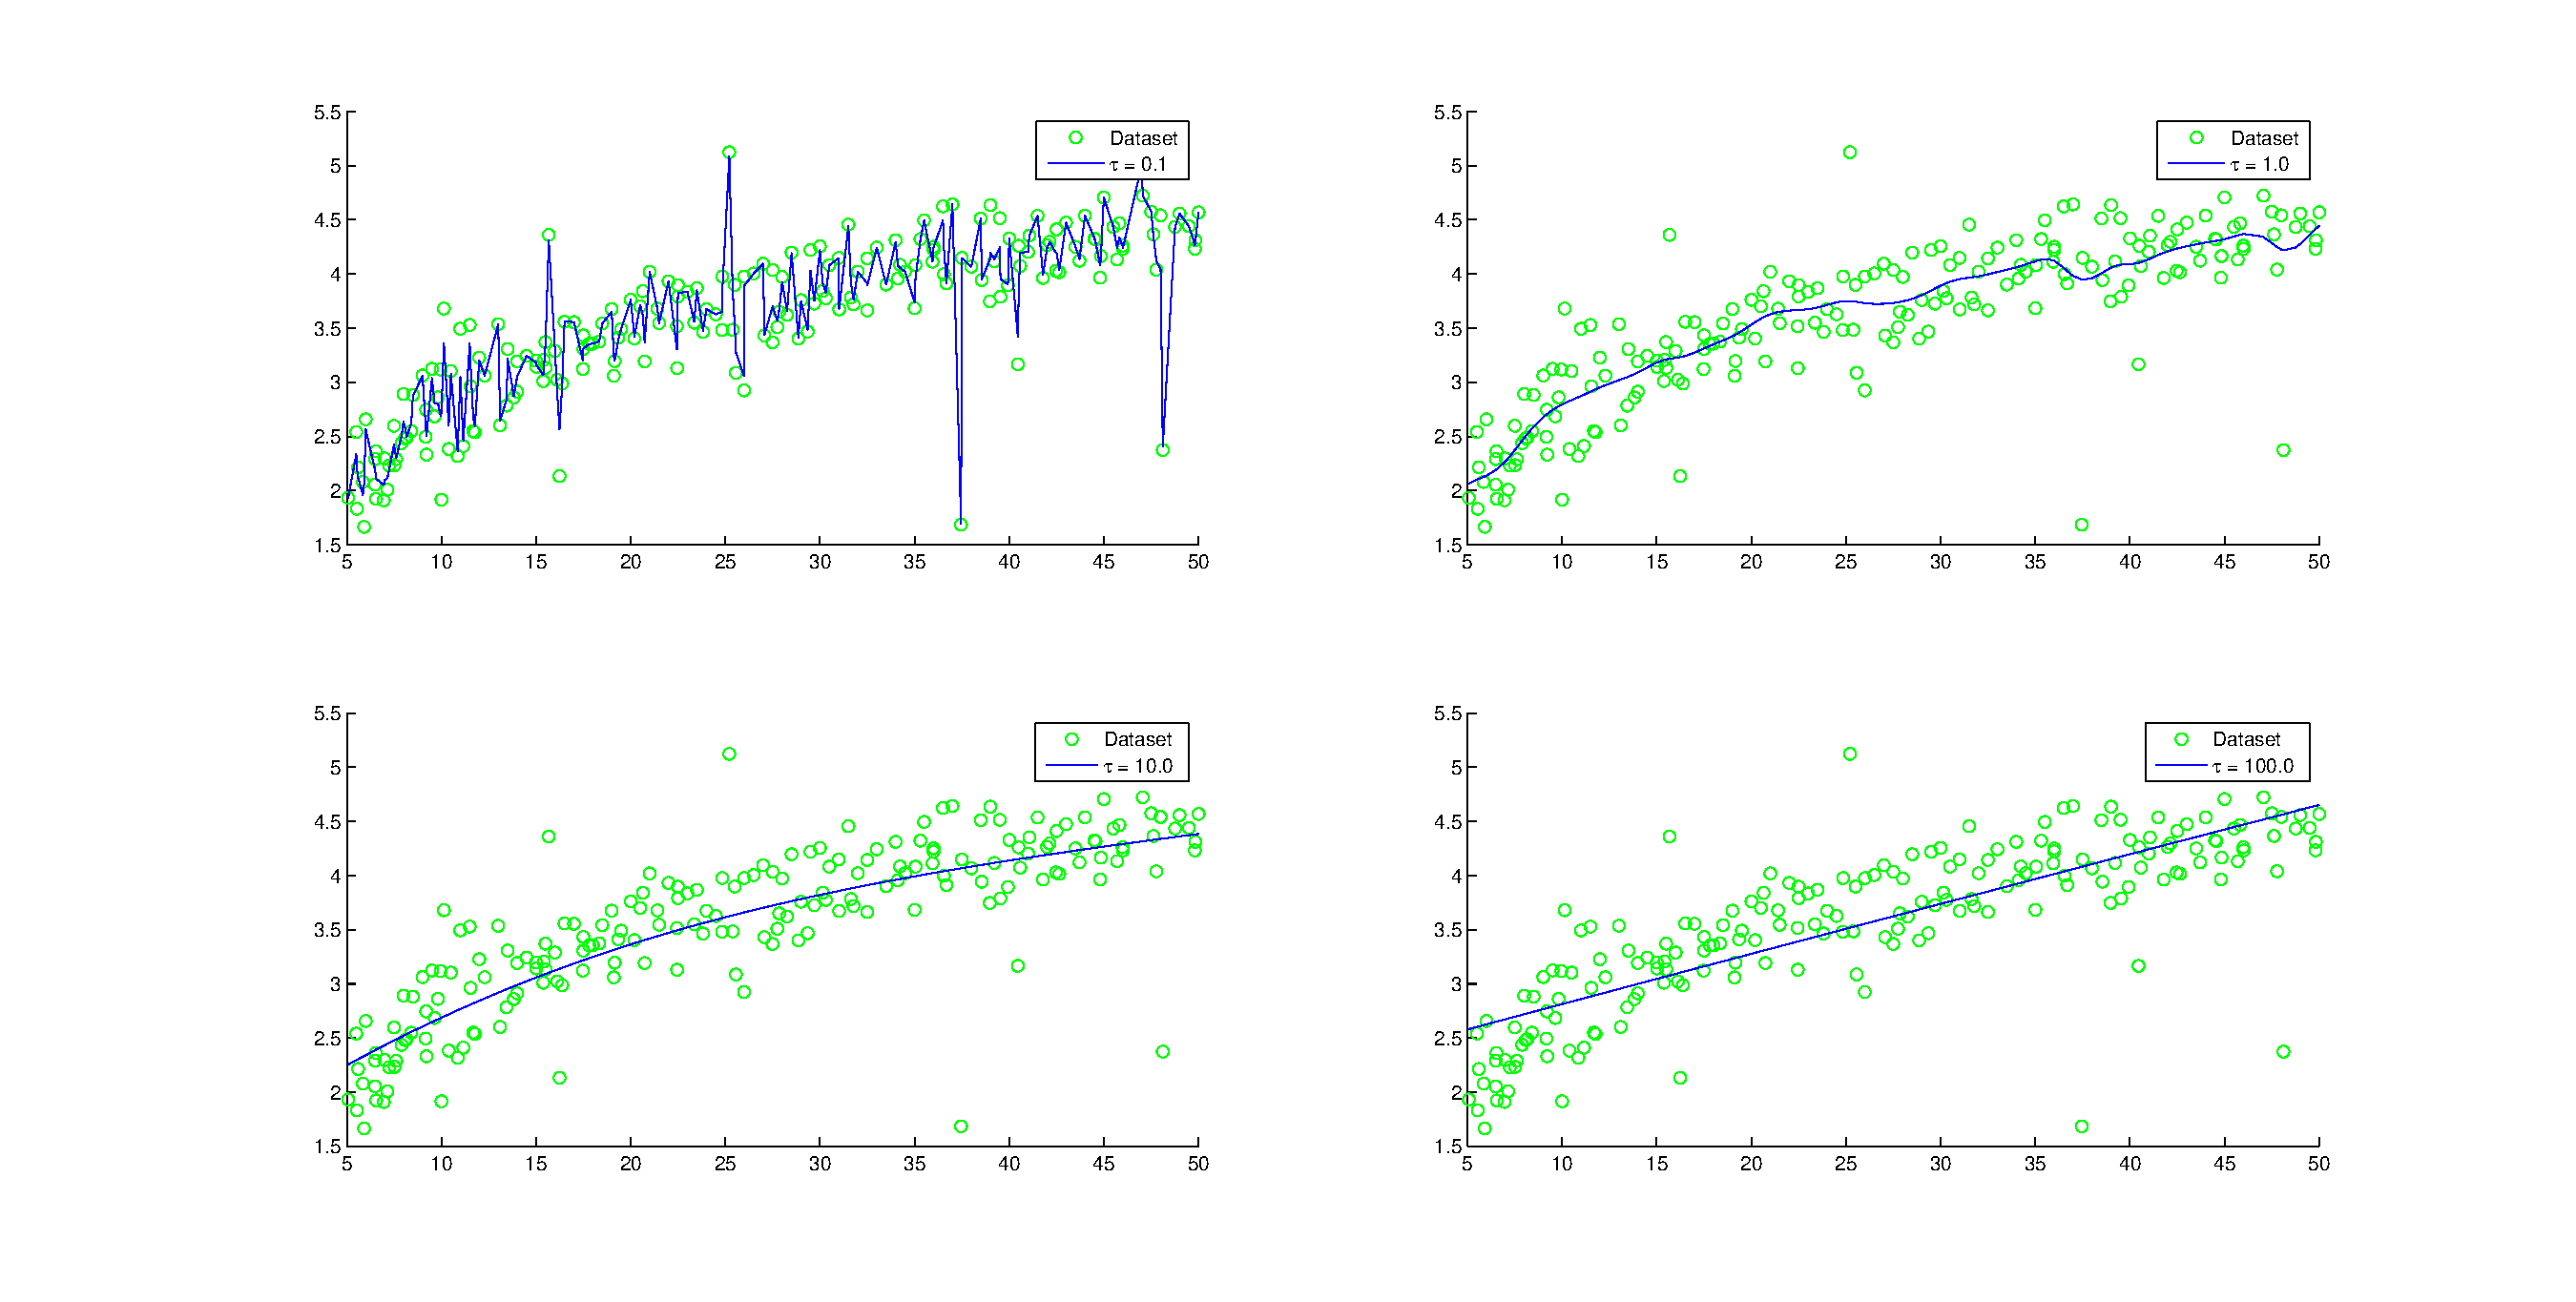
\includegraphics[scale = 0.4]{Q4_e}
						%\end{center}
						\begin{center}
							$\begin{array}{c|c|c|c|c}
								\tau & 0.1 & 1 & 10 & 100 \\
								MSE & 0.0234 & 0.1478 & 0.1650 & 0.1962
							\end{array}$
						\end{center}
					\end {flushleft}
					\noindent\makebox[\linewidth]{\rule{\textwidth}{0.4pt}}
					
				%%%%%%%%%%%                           (f)                                   %%%%%%%%%%%
				\item Discuss what happens when $\tau$ is too small or large.
				
					% Here's the answer
					\noindent\makebox[\linewidth]{\rule{\textwidth}{0.4pt}}
					\begin {flushleft} % Insert the answer
						Obviously, $\displaystyle\lim_{\tau \to \infty} l^{(i)} = 1$. Therefore, the larger $\tau$ we give, 
						the more similar locally weighted linear regressors are to linear regressors. 
						On the other hand, the line we obtain tends to fit the training set when $\tau$ is getting smaller, 
						for minimizing the objective function because the nearer points have greater weights. 
						Therefore, the constant $\tau$ can be regarded as the sensitivity of regressors to the data noise.
					\end {flushleft}
					\noindent\makebox[\linewidth]{\rule{\textwidth}{0.4pt}}
					
					
			\end {enumerate}
	\end {enumerate}

\end{CJK}
\end{document}